\documentclass[tikz,border=2pt]{standalone}
\usepackage{amsmath}
\usetikzlibrary{arrows.meta}
\begin{document}
% Independent risks with sigma_X = sigma_Y = 2 (means 10): standard deviations add like orthogonal legs,
% sigma_{X+Y} = sqrt(2^2+2^2) = sqrt 8 ~ 2.83 < 2+2 = 4, so at alpha = 1 the pooled premium 22.83 is below 24.
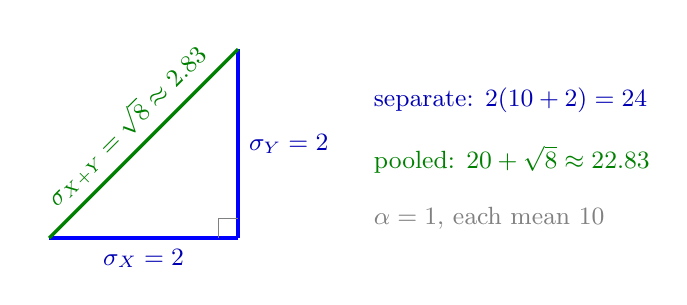
\begin{tikzpicture}[font=\small, >={Latex[length=2mm]}, x=1cm, y=1cm]
  % legs: separate standard deviations
  \draw[blue, very thick] (0,0) -- node[below, blue!70!black] {$\sigma_X=2$} (2.4,0);
  \draw[blue, very thick] (2.4,0) -- node[right, blue!70!black] {$\sigma_Y=2$} (2.4,2.4);
  \draw[gray] (2.15,0) -- (2.15,0.25) -- (2.4,0.25);
  % hypotenuse: pooled standard deviation
  \draw[green!50!black, very thick] (0,0) -- node[above, sloped] {$\sigma_{X+Y}=\sqrt8\approx2.83$} (2.4,2.4);
  % premiums at alpha = 1
  \node[anchor=west, blue!70!black] at (4.0,1.75) {separate: $2(10+2)=24$};
  \node[anchor=west, green!50!black] at (4.0,1.0) {pooled: $20+\sqrt8\approx22.83$};
  \node[anchor=west, gray] at (4.0,0.25) {$\alpha=1$, each mean $10$};
\end{tikzpicture}
\end{document}
